% SEC 6.1
\section[Inner Prod., Length, \& Orth.]{Inner Product, Length, \& Orthogonality}
\name[1.5in]


\begin{boxdef}
	The number $\vect{u}^T\vect{v}$ is called the \textbf{inner product} (or \textbf{dot product}) of $\vect{u}$ and $\vect{v}$. It is written as $\vect{u}\cdot\vect{v}$.
\end{boxdef}
% ADD properties of inner product??


\begin{exercise} % 6.1.2
	Let $\vect{w}=\begin{bmatrix}3\\-1\\-5\end{bmatrix}$ and $\vect{x}=\begin{bmatrix}6\\-2\\3\end{bmatrix}$. Compute the following.
	\begin{multicols}{2}
		\begin{enumerate}[(a)]
			\item $\vect{w}\cdot\vect{w}$
			\vspace{5em}
			\item $\vect{x}\cdot\vect{w}$
			\columnbreak
			\item $\frac{\vect{x}\cdot\vect{w}}{\vect{w}\cdot\vect{w}}$
		\end{enumerate}
	\end{multicols}
	\vspace{5em}
\end{exercise}


\begin{boxdef}
	The \textbf{length} (or \textbf{norm}) of a vector $\vect{v}$ in $\R^n$ is the nonnegative scalar $\|\vect{v}\|$ defined by
	$$ \|\vect{v}\| = \sqrt{\vect{v}\cdot\vect{v}} = \sqrt{v_1^2+v_2^2+\cdots+v_n^2}. $$
	A vector with length 1 is called a \textbf{unit vector}. To create a unit vector $\vect{u}$ from $\vect{v}$, compute $\vect{u}=\frac{1}{\|\vect{v}\|}\vect{v}$. You can think of this as ``dividing $\vect{v}$'' by its length, $\|\vect{v}\|$. This is called \textbf{normalizing} $\vect{v}$. We say the new unit vector $\vect{u}$ is \textbf{in the same direction} as $\vect{v}$.
\end{boxdef}


\begin{exercise} % 6.1.9,11
	For each problem below, find a unit vector in the direction of the given vector. \\
	Hint: You may wish to scale the vector by a positive constant before normalizing. This will not affect the final answer, but it can simplify calculations.
	\begin{multicols}{2}
		\begin{enumerate}[(a)]
			\item $\begin{bmatrix}-30\\40\end{bmatrix}$
			\columnbreak
			\item $\begin{bmatrix}7/4\\1/2\\-1/2\end{bmatrix}$
		\end{enumerate}
	\end{multicols}
\end{exercise}
\vfill


\newpage


\begin{boxdef}
	For $\vect{u}$ and $\vect{v}$ in $\R^n$, the \textbf{distance between $\boldsymbol{\vect{u}}$ and $\boldsymbol{\vect{v}}$}, written $\dist(\vect{u},\vect{v})$, is the length of the vector $(\vect{u}-\vect{v})$. That is,
	\vspace{-1ex}
	$$ \dist(\vect{u},\vect{v}) = \| \vect{u}-\vect{v} \|. $$
\end{boxdef}
\vspace{-1em}
\begin{boxdef}
	Two vectors $\vect{u}$ and $\vect{v}$ are \textbf{orthogonal} if $\vect{u}\cdot\vect{v}=0$. The zero vector, $\vect{0}$, is orthogonal to every vector.
\end{boxdef}


\begin{exercise} % 6.1.16
	The notion of orthogonality is a generalization of perpendicular lines. The vectors $\vect{u}$ and $\vect{v}$ are orthogonal if the distance between $\vect{u}$ and $\vect{v}$ is the same as the distance between $\vect{u}$ and $-\vect{v}$ (see the figure). Given $\vect{u}=\begin{bmatrix}12\\3\\-5\end{bmatrix}$ and $\vect{v}=\begin{bmatrix}2\\-3\\3\end{bmatrix}$, answer the following.

	\begin{enumerate}[(a)]
		\item Determine if $\vect{u}$ and $\vect{v}$ are orthogonal by comparing $\|\vect{u}-\vect{v}\|$ and $\|\vect{u}+\vect{v}\|$.
		
		\hfill
		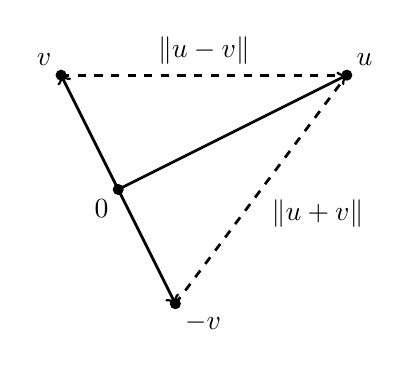
\begin{tikzpicture}[scale=1]
		% Set u and v
		\pgfmathsetmacro{\ux}{4}
		\pgfmathsetmacro{\uy}{2}
		\pgfmathsetmacro{\vx}{-1}
		\pgfmathsetmacro{\vy}{2}
		% Begin Axis
		\begin{axis}[axis lines=none,
		axis x line=center, axis y line=middle, 
		xmin=-2.5, xmax=5.5,
		ymin=-3.5, ymax=3.5,
		scale only axis, axis equal, height=2in,
		grid=major, grid style={line width=.5pt, draw=gray!50, dashed}]
		% Plot vectors
		\fill[black] (0,0) circle (2pt) node[below left, fill=white, rounded corners=0.2cm] {$\vect{0}$};
		\fill[black] (\ux,\uy) circle (2pt) node[above right, fill=white, rounded corners=0.2cm] {$\vect{u}$};
		\fill[black] (\vx,\vy) circle (2pt) node[above left, fill=white, rounded corners=0.2cm] {$\vect{v}$};
		\fill[black] (-\vx,-\vy) circle (2pt) node[below right, fill=white, rounded corners=0.2cm] {$-\vect{v}$};
		\draw[<->,line width=1pt] (\vx,\vy) -- (-\vx,-\vy);
		\draw[->,line width=1pt] (0,0) -- (\ux,\uy);
		\draw[dashed,line width=1pt] (\vx,\vy) -- (\ux,\uy) node[midway, above] {$\|\vect{u}-\vect{v}\|$};
		\draw[dashed,line width=1pt] (-\vx,-\vy) -- (\ux,\uy) node[midway, below right] {$\|\vect{u}+\vect{v}\|$};
		\end{axis}
		\end{tikzpicture}
		\vspace{3em}
		
		\item Determine if $\vect{u}$ and $\vect{v}$ are orthogonal by computing $\vect{u}\cdot\vect{v}$.
		\vspace{5em}
	\end{enumerate}
\end{exercise}


\begin{boxdef}
	If $\vect{z}$ is orthogonal to every vector in a subspace $W$, then we say $\vect{z}$ is \textbf{orthogonal} to $W$. The set of all $\vect{z}$ orthogonal to $W$ is called the \textbf{orthogonal complement} of $W$, denoted $W^\perp$. A vector $\vect{z}$ is in $W^\perp$ if, and only if, $\vect{z}$ is orthogonal to every vector in a spanning set for $W$.
\end{boxdef}

\begin{exercise} % 6.1.Custom
	Suppose $W$ is spanned by the set $\left\{ \begin{bmatrix}-4\\1\\-2\\6\end{bmatrix},\begin{bmatrix}2\\-5\\-1\\4\end{bmatrix} \right\}$. Is $\vect{u}=\begin{bmatrix}3\\2\\-5\\0\end{bmatrix}$ in $W^\perp$?
\end{exercise}
\vfill


\newpage


% SEC 6.2
\section{Orthogonal Sets}
\name

\begin{boxme}
	A set of vectors $\vectsetvp$ in $\R^n$ is said to be an \textbf{orthogonal set} if each pair of distinct vectors from the set is orthogonal, that is, if $\vect{v}_i\cdot\vect{v}_j=0$ whenever $i\neq j$.
\end{boxme}


\begin{exercise} % 6.2.4 (scaled)
	Determine if the set $\{\vect{u}_1,\vect{u}_2,\vect{u}_3\}$ is orthogonal.
	$$ \vect{u}_1 = \begin{bmatrix}2\\-2\\1\\2\end{bmatrix}, \quad
	\vect{u}_2 = \begin{bmatrix}-1\\4\\-4\\7\end{bmatrix}, \quad
	\vect{u}_3 = \begin{bmatrix}4\\7\\6\\0\end{bmatrix} $$
\end{exercise}
\vfill


\begin{boxthm}
	\textbf{Theorem 6.4.} \\
	If $S=\vectset[u]{1}{p}$ is an orthogonal set of nonzero vectors in $\R^n$, then $S$ is linearly independent and hence is a basis for the subspace spanned by $S$.
\end{boxthm}
\vspace{-1em}
\begin{boxthm}
	\textbf{Theorem 6.5.} \\
	Let $\vectset[u]{1}{p}$ be an orthogonal basis for a subspace $W$ of $\R^n$. For each $\vect{y}$ in $W$, the weights in the linear combination
	\vspace{-1ex}
	$$ \vect{y} = c_1\vect{u}_1+\cdots+c_p\vect{u}_p $$
	are given by 
	\vspace{-1ex}
	$$ c_j = \frac{\vect{y}\cdot\vect{u}_j}{\vect{u}_j\cdot\vect{u}_j} \qquad
	(\text{for } j=1,\ldots,p). $$
\end{boxthm}


\begin{exercise} % 6.2.10 (Don't have to check orthogonality)
	The set $\{\vect{u}_1,\vect{u}_2,\vect{u}_3\}$ is orthogonal. By Theorem 6.4 (and Theorem 2.15 or 4.12, The Basis Theorem), the set is a basis for $\R^3$. Write $\vect{x}$ as a linear combination of the basis vectors: $\vect{x} = c_1\vect{u}_1 + c_2\vect{u}_2 + c_3\vect{u}_3$.
	$$ \vect{u}_1 = \begin{bmatrix}2\\-2\\0\end{bmatrix}, \quad
	\vect{u}_2 = \begin{bmatrix}3\\3\\-1\end{bmatrix}, \quad
	\vect{u}_3 = \begin{bmatrix}1\\1\\6\end{bmatrix}, \quad
	\vect{x} = \begin{bmatrix}4\\-3\\1\end{bmatrix} $$
\end{exercise}
\vfill


\newpage


\begin{boxdef}
	Suppose $\vect{u}$ and $\vect{y}$ are given. It will be useful to write $\vect{y}=\yhat+\vect{z}$ where $\yhat$ is some scalar multiple of $\vect{u}$ and $\vect{z}$ is orthogonal to $\vect{u}$. The vector $\yhat$ is called the \textbf{orthogonal projection of $\vect{y}$ onto $\vect{u}$}, and the vector $\vect{z}$ is called the \textbf{component of $\vect{y}$ orthogonal to $\vect{u}$}.
	\vspace{-1em}
	\begin{multicols}{2}
		\begin{center}
		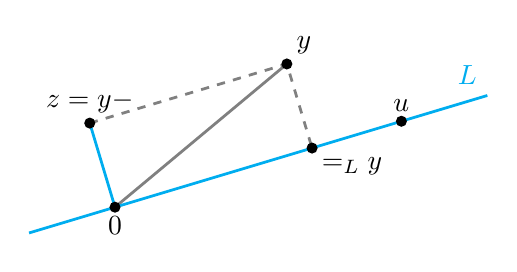
\begin{tikzpicture}[scale=1]
		% Set u and v
		\pgfmathsetmacro{\ux}{5}
		\pgfmathsetmacro{\uy}{1.5}
		\pgfmathsetmacro{\yx}{3}
		\pgfmathsetmacro{\yy}{2.5}
		\pgfmathparse{\yx*\ux+\yy*\uy}
		\pgfmathsetmacro{\ydotu}{\pgfmathresult}
		\pgfmathparse{\ux*\ux+\uy*\uy}
		\pgfmathsetmacro{\udotu}{\pgfmathresult}
		\pgfmathparse{\ydotu/\udotu*\ux}
		\pgfmathsetmacro{\yhatx}{\pgfmathresult}
		\pgfmathparse{\ydotu/\udotu*\uy}
		\pgfmathsetmacro{\yhaty}{\pgfmathresult}
		\pgfmathparse{\yx-\yhatx}
		\pgfmathsetmacro{\zx}{\pgfmathresult}
		\pgfmathparse{\yy-\yhaty}
		\pgfmathsetmacro{\zy}{\pgfmathresult}
		% Begin Axis
		\begin{axis}[axis lines=none,
		axis x line=center, axis y line=middle,
		xmin=-.5, xmax=5.5,
		ymin=-3.5, ymax=6.5,
		%	xtick={-3,...,5}, ytick={-3,...,7},
		%	xticklabels={,,}, yticklabels={,,},
		scale only axis, axis equal, % height=2in,
		gray, grid=major, grid style={line width=.5pt, draw=gray!50, dashed}]
		% Set Coordinates
		\coordinate (O) at (0,0);
		\coordinate (U) at (\ux,\uy);
		\coordinate (Y) at (\yx,\yy);
		\coordinate (YHAT) at (\yhatx,\yhaty);
		\coordinate (Z) at (\zx,\zy);
		% Connect Vectors
		\draw[line width=1pt] (O) -- (Y);
		\draw[cyan, line width=1pt] (O) -- (Z);
		\draw[dashed, line width=1pt] (Z) -- (Y) -- (YHAT);
		% Plot u and Span{u}
		\addplot[-, cyan, line width=1pt, domain=-1.5:6.5]{(\uy/\ux)*x} node[above left] {$L$};
		% Plot vectors
		\fill[black] (O) circle (2pt) node[below] {$\vect{0}$};
		\fill[black] (U) circle (2pt) node[above] {$\vect{u}$};
		\fill[black] (Y) circle (2pt) node[above right] {$\vect{y}$};
		\fill[black] (YHAT) circle (2pt) node[below right] {$\yhat=\proj_L\vect{y}$};
		\fill[black] (Z) circle (2pt) node[above] {$\vect{z}=\vect{y}-\yhat$};
		% ADD RIGHT ANGLE
		\end{axis}
		\end{tikzpicture}
		\end{center}

		\columnbreak
		
		If we let $L=\Span\{\vect{u}\}$, then we write
		$$ \yhat = \proj_L\vect{y} = \frac{\vect{y}\cdot\vect{u}}{\vect{u}\cdot\vect{u}}\vect{u} $$
	\end{multicols}
\end{boxdef}


\begin{exercise} % 6.2.12
	\begin{enumerate}[(a)]
		\item Compute the orthogonal projection of $\vect{y}=\begin{bmatrix}-4\\3\end{bmatrix}$ onto the line through $\vect{u}=\begin{bmatrix}-1\\4\end{bmatrix}$ and the origin.
		\vfill
		
		\item Using part (a), how could you compute the shortest distance from $\vect{y}$ to $L=\Span{\vect{u}}$?
		\vspace{3em}
	\end{enumerate}
\end{exercise}


\begin{boxdef}
	A set $\vectsetvp$ is an \textbf{orthonormal} if it is an orthogonal set of unit vectors. If $W=\Span\vectsetvp$, then the set is an \textbf{orthonormal basis} for $W$.
\end{boxdef}

\begin{exercise} % 6.2.17
	Determine if the set of vectors is orthonormal. If the set is only orthogonal, normalize the vectors to produce an orthonormal set.
	$$ \vect{u}_1 = \begin{bmatrix}2/3\\1/3\\1/3\end{bmatrix}, \quad
	\vect{u}_2 = \begin{bmatrix}1/\sqrt{5}\\0\\-2/\sqrt{5}\end{bmatrix} $$
\end{exercise}
\vfill


\newpage


% SEC 6.3
\section{Orthogonal Projections}
\name

\begin{boxthm}
	\textbf{Theorem 6.8.}
	\textbf{The Orthogonal Decomposition Theorem} \\
	Let $W$ be a subspace of $\R^n$. Then each $\vect{y}$ in $\R^n$ can be written uniquely in the form
	$ \vect{y} = \yhat+\vect{z} $
	where $\yhat$ is in $W$ and $\vect{z}$ is in $W^\perp$. In fact, if $\vectset[u]{1}{p}$ is any orthogonal basis of $W$, then
	$$ \yhat = \frac{\vect{y}\cdot\vect{u}_1}{\vect{u}_1\cdot\vect{u}_1}\vect{u}_1 + \cdots + \frac{\vect{y}\cdot\vect{u}_p}{\vect{u}_p\cdot\vect{u}_p}\vect{u}_p \qquad \text{and} \qquad \vect{z}=\vect{y}-\yhat. $$
	The vector $\yhat$ is called the \textbf{orthogonal projection of $\boldsymbol{\vect{y}}$ onto $\boldsymbol{W}$}, and the vector $\vect{z}$ is called the \textbf{component of $\boldsymbol{\vect{y}}$ orthogonal to $\boldsymbol{W}$}.
\end{boxthm}


\begin{exercise} % 6.3.5
	Verify that $\{\vect{u}_1,\vect{u}_2\}$ is an orthogonal set, and then find $\yhat$, the orthogonal projection of $\vect{y}$ onto $\Span\{\vect{u}_1,\vect{u}_2\}$. Hint: If you do the problem correctly, $\yhat$ has all integer entries.
	$$ \vect{y} = \begin{bmatrix}-1\\3\\6\end{bmatrix}, \quad
	\vect{u}_1 = \begin{bmatrix}-5\\-1\\-2\end{bmatrix}, \quad
	\vect{u}_2 = \begin{bmatrix}1\\-1\\-2\end{bmatrix}$$
\end{exercise}
\vfill


\begin{exercise} % 6.3.1
	Write $\vect{x}$ as the sum of two vectors, one in $\Span\{\vect{u}_1,\vect{u}_2,\vect{u}_3\}$ and the other in $\Span\{\vect{u}_4\}$. You may assume $\{\vect{u}_1,\vect{u}_2,\vect{u}_3,\vect{u}_4\}$ is an orthogonal basis for $\R^4$.
	$$ \vect{u}_1 = \begin{bmatrix}0\\1\\-4\\-1\end{bmatrix}, \quad
	\vect{u}_2 = \begin{bmatrix}3\\5\\1\\1\end{bmatrix}, \quad
	\vect{u}_3 = \begin{bmatrix}1\\0\\1\\-4\end{bmatrix}, \quad
	\vect{u}_4 = \begin{bmatrix}5\\-3\\-1\\1\end{bmatrix}, \quad
	\vect{x} = \begin{bmatrix}10\\-8\\2\\0\end{bmatrix}$$
	Hint: You could compute the orthogonal projections of $\vect{x}$ onto $\Span\{\vect{u}_1,\vect{u}_2,\vect{u}_3\}$ and $\Span\{\vect{u}_4\}$, but there is a much quicker method using Theorem 6.8. If we let $\xhat$ be the orthogonal projection of $\vect{x}$ onto $W=\Span\{\vect{u}_4\}$. Then $\vect{z}=\vect{x}-\xhat$ is in $W^\perp=\Span\{\vect{u}_1,\vect{u}_2,\vect{u}_3\}$. So $\vect{x}=\xhat+\vect{z}$ will be the sum you want.
\end{exercise}
\vfill


\newpage


\begin{boxthm}
	\textbf{Theorem 6.9.}
	\textbf{The Best Approximation Theorem} \\
	Let $W$ be a subspace of $\R^n$, let $\vect{y}$ be any vector in $\R^n$, and let $\yhat$ be the orthogonal projection of $\vect{y}$ onto $W$. Then $\yhat$ is the closest point in $W$ to $\vect{y}$, in the sense that
	$$ \|\vect{y}-\yhat\| < \|\vect{y}-\vect{v}\| $$
	for all $\vect{v}$ in $W$ distinct from $\yhat$. The vector $\yhat$ is \textbf{the best approximation to $\boldsymbol{\vect{y}}$ by elements of $\boldsymbol{W}$}.
\end{boxthm}


\begin{exercise} % 6.3.12
	Find the closest point to $\vect{y}$ in the subspace $W$ spanned by $\vect{v}_1$ and $\vect{v}_2$. Assume $\vect{v}_1$ and $\vect{v}_2$ are orthogonal.
	$$ \vect{y} = \begin{bmatrix}3\\-1\\1\\13\end{bmatrix}, \quad
	\vect{v}_1 = \begin{bmatrix}1\\-2\\-1\\2\end{bmatrix}, \quad
	\vect{v}_2 = \begin{bmatrix}-4\\1\\0\\3\end{bmatrix} $$
\end{exercise}
\vfill


\begin{boxthm}
	\textbf{Theorem 6.10.} \\
	If $\vectset[u]{1}{p}$ is an orthonormal basis for a subspace $W$ of $\R^n$, then
	$$ \proj_W\vect{y} = (\vect{y}\cdot\vect{u}_1)\vect{u}_1 + (\vect{y}\cdot\vect{u}_2)\vect{u}_2 + \cdots + (\vect{y}\cdot\vect{u}_p)\vect{u}_p. $$
	If $U=\begin{bmatrix}\vect{u}_1&\vect{u}_2&\cdots&\vect{u}_p\end{bmatrix}$, then
	$ \proj_W\vect{y} = UU^T\vect{y}$ for all $\vect{y}$ in $\R^n$.
\end{boxthm}


\begin{exercise} % 6.3.17
	Let $\vect{y}=\begin{bmatrix}4\\8\\1\end{bmatrix}$, $\vect{u}_1=\begin{bmatrix}2/3\\1/3\\2/3\end{bmatrix}$, $\vect{u}_2=\begin{bmatrix}-2/3\\2/3\\1/3\end{bmatrix}$, and $W=\Span\{\vect{u}_1,\vect{u}_2\}$. You may assume $\{\vect{u}_1,\vect{u}_2\}$ is orthonormal.
	\begin{enumerate}[(a)]
		\item Let $U=\begin{bmatrix}\vect{u}_1&\vect{u}_2\end{bmatrix}$ and compute $UU^T$.
		
		$UU^T = \begin{bmatrix}2/3&-2/3\\1/3&2/3\\2/3&1/3\end{bmatrix}
		\begin{bmatrix}2/3&1/3&2/3\\-2/3&2/3&1/3\end{bmatrix}=$
		\vspace{2em}
		\item Compute $\proj_W\vect{y}=UU^T\vect{y}$.
		\vspace{1in}
	\end{enumerate}
\end{exercise}


\newpage


% SEC 6.4
\section{The Gram-Schmidt Process}
\name

\begin{boxthm}
	\textbf{Theorem 6.11.}
	\textbf{The Gram-Schmidt Process} \\
	Given a basis $\vectset[x]{1}{p}$ for a nonzero subspace $W$ of $\R^n$, define
	\vspace{-1ex}
	\begin{align*}
	\vect{v}_1 &= \vect{x}_1 \\
	\vect{v}_2 &= \vect{x}_2 - \frac{\vect{x}_2\cdot\vect{v}_1}{\vect{v}_1\cdot\vect{v}_1}\vect{v}_1 \\
	\vect{v}_3 &= \vect{x}_3 - \frac{\vect{x}_3\cdot\vect{v}_1}{\vect{v}_1\cdot\vect{v}_1}\vect{v}_1 - \frac{\vect{x}_3\cdot\vect{v}_2}{\vect{v}_2\cdot\vect{v}_2}\vect{v}_2 \\
	&\vdots \\
	\vect{v}_p &= \vect{x}_p - \frac{\vect{x}_p\cdot\vect{v}_1}{\vect{v}_1\cdot\vect{v}_1}\vect{v}_1 - \frac{\vect{x}_p\cdot\vect{v}_2}{\vect{v}_2\cdot\vect{v}_2}\vect{v}_2 - \ldots -  \frac{\vect{x}_p\cdot\vect{v}_{p-1}}{\vect{v}_{p-1}\cdot\vect{v}_{p-1}}\vect{v}_{p-1}.
	\end{align*}
	Then $\vectsetvp$ is an orthogonal basis for $W$, and $\Span\vectset{1}{k} = \Span\vectset[x]{1}{k}$ for $k\leq p$.
\end{boxthm}


\begin{exercise} % 6.4.3
	The set $\{\vect{x}_1,\vect{x}_2\}$ is a basis for a subspace $W$. Use the Gram-Schmidt process to produce an orthogonal basis for $W$. Hint: Scaling vectors before you begin may simplify calculations.
	
	\vspace{1em}
	$ \vect{x}_1 = \begin{bmatrix}2\\-5\\4\end{bmatrix}, \quad
	\vect{x}_2 = \begin{bmatrix}6\\-6\\3\end{bmatrix} $
\end{exercise}
\vfill


\begin{exercise} % 6.4.10 (altered)
	A matrix $A$ with linearly independent columns is given below. Find an orthogonal basis for the column space of $A$. Note that columns 1 and 2 are already orthogonal. Hint: Recall that one possible basis for $\Col A$ consists of the pivot columns of $A$.
	
	\vspace{1em}
	$ A = \begin{bmatrix}-1&1&3\\3&0&1\\2&1&3\\1&-1&-1\end{bmatrix} $
\end{exercise}
\vfill


\newpage


\begin{exercise} % 6.4.8
	The set $\{\vect{v}_1,\vect{v}_2\}$ is an orthogonal basis for a subspace $W$. Find an orthonormal basis for $W$. Hint: Since scaling vectors does not affect orthogonality, you may wish to scale $\vect{v}_1$ and $\vect{v}_2$ before normalizing.
	
	\vspace{1em}
	$ \vect{v}_1 = \begin{bmatrix}2\\-6\\4\end{bmatrix}, \quad
	\vect{v}_2 = \begin{bmatrix}-5\\-5\\-5\end{bmatrix} $
\end{exercise}
\vspace{1.75in}


\begin{boxthm}
	\textbf{Theorem 6.12.}
	\textbf{The $\boldsymbol{QR}$ Factorization} \\
	If $A$ is an $m\times n$ matrix with linearly independent columns, then $A$ can be factored as $A=QR$, where $Q$ is an $m\times n$ matrix whose columns form an orthonormal basis for $\Col A$ and $R$ is an $n\times n$ upper triangular invertible matrix with positive entries on its diagonal.
\end{boxthm}
\vspace{-1em}
\begin{boxme}
	To produce $Q$, orthogonalize and normalize the columns of $A$, i.e., apply the Gram-Schmidt process (with normalization) to the columns of $A$. To produce $R$, use the following:
	\vspace{-1em}
	\begin{align*}
	QR &= A \\
	Q^TQR &= Q^TA \\
	IR &= Q^TA &\text{(By Thm 6.6, since $Q$ has orthonormal columns, $Q^TQ=I$)}\\
	R &= Q^TA
	\end{align*}
\end{boxme}


\begin{exercise} % 6.4.14
	The columns of $Q$ were obtained by applying the Gram-Schmidt process (with normalization) to the columns of $A$. Find an upper triangular matrix $R$ such that $A=QR$.
	
	\vspace{1em}
	$ A= \begin{bmatrix}-2&-3\\5&7\\-2&-2\\-4&-1\end{bmatrix}, \quad
	Q= \begin{bmatrix}-2/7&-1/\sqrt{14}\\5/7&2/\sqrt{14}\\-2/7&0\\-4/7&3/\sqrt{14}\\\end{bmatrix}$
%	\begin{align*}
%	A &= \begin{bmatrix}-2&-3\\5&7\\-2&-2\\-4&-1\end{bmatrix} &
%	Q &= \begin{bmatrix}-2/7&-1/\sqrt{14}\\5/7&2/\sqrt{14}\\-2/7&0\\-4/7&3/\sqrt{14}\\\end{bmatrix}
%	\end{align*}
\end{exercise}
\vfill


\newpage


% SEC 6.5
\section{Least-Squares Problems}
\name

%\begin{boxdef}
%If $A$ is $m\times n$ and $\vect{b}$ is in $\R^m$, a \textbf{least-squares solution} of $\Axb$ is an $\xhat$ in $\R^n$ such that
%\vspace{-1ex}
%$$ \|\vect{b}-A\xhat\| \leq \|\vect{b}-A\vect{x}\| \qquad
%\text{for all $\vect{x}$ in $\R^n$.} $$
%\end{boxdef}

\begin{boxthm}
	\textbf{Theorem 6.13.} \\
	The set of least-squares solutions of $\Axb$ coincides with the nonempty set of solutions of the normal equations $\NormEq$.
\end{boxthm}


\begin{exercise} % 6.5.5
	Describe all the least-squares solutions of the equation $\Axb$.
	\begin{multicols}{2}
		$ A = \begin{bmatrix}1&1&0\\1&1&0\\1&0&1\\1&0&1\end{bmatrix}, 
		\vect{b} = \begin{bmatrix}2\\6\\5\\1\end{bmatrix} $
		\begin{enumerate}[(a)]
			\item Compute $A^TA$ and $A^T\vect{b}$. \\
			$ A^TA = \begin{bmatrix}1&1&1&1\\1&1&0&0\\0&0&1&1\end{bmatrix} \begin{bmatrix}1&1&0\\1&1&0\\1&0&1\\1&0&1\end{bmatrix} = $
			
			\vspace{2em}
			$ A^T\vect{b} = \begin{bmatrix}1&1&1&1\\1&1&0&0\\0&0&1&1\end{bmatrix} \begin{bmatrix}2\\6\\5\\1\end{bmatrix} = $
			\columnbreak
			\item Solve $\NormEq$. \\
			(You may use a calculator or computer)
		\end{enumerate}
	\end{multicols}
\end{exercise}
\vspace{2em}


\begin{boxthm}
	\textbf{Theorem 6.14.} \\
	Let $A$ be an $m\times n$ matrix. The following statements are logically equivalent:
	\vspace{-1ex}
	\begin{enumerate}[(a)]\itemsep=0em
		\item The equation $\Axb$ has a unique least-squares solution for each $\vect{b}$ in $\R^m$.
		\item The columns of $A$ are linearly independent.
		\item The matrix $A^TA$ is invertible.
	\end{enumerate}
	\vspace{-1ex}
	When these statements are true, the least-squares solution $\xhat$ is given by
	$ \xhat = \left(A^TA\right)^{-1}A^T\vect{b}. $
\end{boxthm}


\begin{exercise} % 6.5.1
	Find a least-squares solution of $\Axb$. Use Theorem 6.14 if applicable. \par
	$ A = \begin{bmatrix}-1&2\\2&-3\\-1&3\end{bmatrix}, 
	\vect{b} = \begin{bmatrix}16\\4\\8\end{bmatrix} $
	
	\begin{multicols}{2}
	\begin{align*}
	A^TA &= \begin{bmatrix}-1&2&-1\\2&-3&3\end{bmatrix}
	\begin{bmatrix}-1&2\\2&-3\\-1 &3\end{bmatrix} \\
	&= \begin{bmatrix}6&-11\\-11&22\end{bmatrix} \\[1em]
	A^T\vect{b} &= \begin{bmatrix}-1&2&-1\\2&-3&3\end{bmatrix} \begin{bmatrix}16\\4\\8\end{bmatrix} = \begin{bmatrix}-16\\44\end{bmatrix}
	\end{align*}
	
	\columnbreak
	\end{multicols}
\end{exercise}
\vfill


\newpage


\begin{exercise} % 6.5.10
	Let $ A = \begin{bmatrix}1&2\\-1&4\\1&2\end{bmatrix} $ and $ \vect{b} = \begin{bmatrix}2\\-1\\6\end{bmatrix} $.
	\begin{enumerate}[(a)]
		\item Find the orthogonal projection of $\vect{b}$ onto $\Col A$. Note that the columns of $A$ are linearly independent and orthogonal, so you already have an orthogonal basis for $\Col A$.
		\vspace{1.75in}
		\item Use your calculations in part (a) to find a least-squares solution of $\Axb$. \par Hint: Think of the entries of $\vect{x}$ as weights for a linear combination of the columns of $A$.
		\vspace{4em}
	\end{enumerate}
\end{exercise}


\begin{boxthm}
	\textbf{Theorem 6.15.} \\
	Given an $m\times n$ matrix $A$ with linearly independent columns, let $A=QR$ be a $QR$ factorization of $A$ as in Theorem 6.12. Then, for each $\vect{b}$ in $\R^m$, the equation $\Axb$ has a unique least-squares solution, given by
	\vspace{-1em}
	\begin{align*}
	\xhat &= R^{-1}Q^T\vect{b}. &
	(\text{Numerical Note: it is usually much quicker to solve } R\xhat = Q^T\vect{b}.)
	\end{align*}
\end{boxthm}


\begin{exercise} % 6.5.15
	Use the factorization $A=QR$ given below to find the least-squares solution of $\Axb$.
	\begin{align*}
	A &= \begin{bmatrix}2&3\\2&4\\1&1\end{bmatrix} =
	\begin{bmatrix}2/3&-1/3\\2/3&2/3\\1/3&-2/3\end{bmatrix}
	\begin{bmatrix}3&5\\0&1\end{bmatrix} &
	\vect{b} &= \begin{bmatrix}6\\3\\9\end{bmatrix}
	\end{align*}
	\begin{enumerate}[(a)]
		\item Compute $Q^T\vect{b}$. \par
		$ Q^T\vect{b}= \begin{bmatrix}2/3&2/3&1/3\\-1/3&2/3&-2/3\end{bmatrix}
		\begin{bmatrix}6\\3\\9\end{bmatrix} = $
		\vspace{2em}
		\item Solve $R\xhat=Q^T\vect{b}$ via back-substitution.
		\vspace{1in}
	\end{enumerate}
\end{exercise}


\newpage
